\chapter{\label{chap:experimentation-and-results}Experimentação e Resultados Obtidos}

\todoin[caption={Experimentos Realizados}, color=cyan!60] {
    Experimentos:

	\begin{itemize}
        \item Inputs: visão, bias
        \item Outputs:
        \begin{itemize}
            \item convencionais: MOVIMENTACAO, PULO
            \item especificos: MOVIMENTACAO, PULO, EXTRA (depende do cenario)
        \end{itemize}
		\item Experimento \#1:fitness: AM, WAM, HM. Mapas: \textbf{easy}.
		\item Checkpoint: definir a fitness (WAM).

		\item Experimento \#2: rodar mapa medium com WAM
		\item Checkpoint: não vai funcionar (local ótimo)
		\item Checkpoint: adicionar novo input: \textbf{obstaculos}

		\item Experimento \#3: rodar mapa medium com WAM e novo input
		\item Checkpoint: funcionou, mas é um pouco problemático

		\item Experimento \#4: fitness exploratória (EX) com novo input
		\item Checkpoint: funcionou melhor

		\item Experimento \#5: janela de visão: 5x5, 7x7. Mapas: \textbf{medium}.
        \item Checkpoint: definir o tamanho da janela de visão.

        \item Experimento \#6: configurações de mutação. Mapas: \textbf{medium}.
        \item Checkpoint: definir configurações de mutação do NEAT.

		\item Experimento \#7: rodar mapa hard com as configurações definidas
		\item Checkpoint: ???

		\item Experimento \#7: experimentos nos cenários específicos
		\item Checkpoint: ???

		\item BONUS: fitness com A* ao invés de Manhattan Distance
		\item Checkpoint: ???
    \end{itemize}
	
    }

\todoin[caption={Detalhes}]{Introdução desse capítulo}


%----------
\section{\label{section:environment}Ambiente de Execução}
O capítulo \ref{chap:development} explica que faremos a execução do jogo em um
ambiente dedicado, utilizando o sistema operacional \textit{Linux}. Para isso,
utilizamos a plataforma \textit{Digital
Ocean}\footnote{https://www.digitalocean.com/}, que facilita a criação de uma
máquina para uso nesse trabalho. Além disso, essa plataforma permite alterar as
configurações -- quantidade de memória, número de processadores e quantidade de
armazenamento -- das máquina a qualquer momento, o que nos permitiu testar
diferentes configurações para o nosso problema.

Conforme explicado na seção \ref{sub:virtual-display}, fazemos o uso do
\textit{XVFB} para permitir a execução do jogo em um \textit{display} virtual. A
utilização de um \textit{display} virtual significa que necessitamos de uma
quantidade razoável de memória na máquina, sendo este um dos recursos mais
importantes para nós. Embora façamos a gravação de algumas informações em disco,
tratam-se apenas de arquivos de texto, que não ocupam uma grande quantidade de
espaço. Tendo isso em consideração, optamos por utilizar \textbf{3} máquinas,
com as configurações exibidas a seguir:

\begin{description}
    \item [Sistema Operacional] Ubuntu 16.04 - 64 \textit{bits}
    \item [Número de Processadores] 4
    \item [Modelo do Processador] Intel(R) Xeon(R) CPU E5-2630L v2 @ 2.40GHz
    \item [Quantidade de Memória] 4GB
    \item [Tipo de Disco] SSD
    \item [Quantidade de Disco] 60GB
\end{description}

Para automatizar o processo de configuração dessas máquinas, fizemos um
\textit{script} de instalação\footnote{https://github.com/famw/provisioning} de
todas as dependências para executar o projeto. Isto faz com que seja fácil
configurar uma nova máquina capaz de executar o treinamento dos agentes.


%----------
\section{\label{section:experiments}Experimentos Realizados}

\subsection{\label{section:fitness-experiment}Escolha da Função de Aptidão}

\todoin[caption={Citar capítulo de modelagem}] {
    Citar capítulo de modelagem.
}

Conforme vimos no capítulo XYZ. A função de aptidão é o que determina a
\textbf{qualidade} da execução de um agente inteligente que utiliza algoritmos
genéticos. Portanto, é de extrema relevância experimentarmos diferentes valores
de aptidão para descobrirmos qual o que se encaixa melhor no nosso problema.

Assim, fizemos a execução do \textit{bot} no cenário \textbf{fácil} (Figura
\ref{fig:level1}, Capítulo \ref{chap:scenarios}) com três diferentes funções de
aptidão: \textbf{média aritmética}, \textbf{média aritmética ponderada} e
\textbf{média harmônica}. Obtivemos os resultados apresentados na Figura
\ref{fig:fitness-experiment}.

\begin{figure}[H]
\centering
	\begin{subfigure}[b]{0.4\textwidth}
        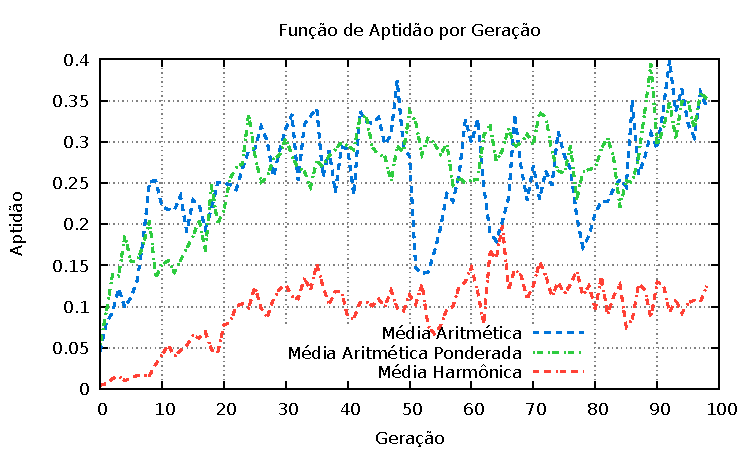
\includegraphics[width=\textwidth]{fig/fitness-value-comparison.pdf}
        \caption{Valor de aptidão em função do número de gerações para as
        diferentes funções de aptidão escolhidas.}
	\end{subfigure}
	\begin{subfigure}[b]{0.4\textwidth}
        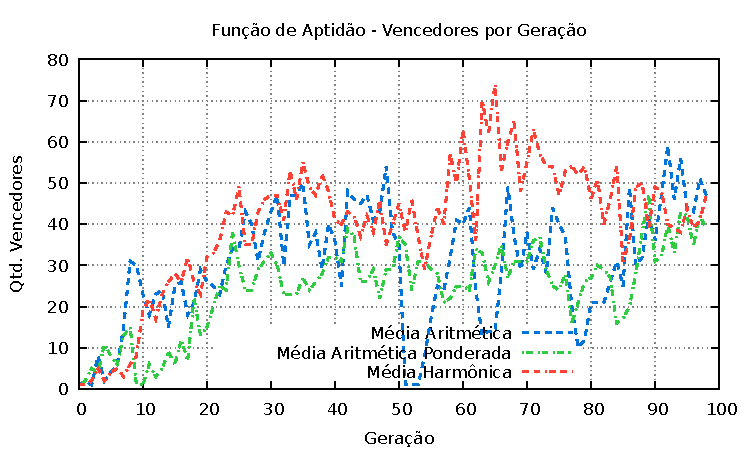
\includegraphics[width=\textwidth]{fig/fitness-winners-comparison.pdf}
        \caption{Número de organismos vencedores por geração para as diferentes
        funções de aptidão escolhidas.}
	\end{subfigure}

    \caption{Resultado da execução do cenário fácil com diferentes funções de
    aptidão.}
	\label{fig:fitness-experiment}
\end{figure}

Através da análise dos resultados, podemos ver que a \textbf{média
artimética} e a \textbf{média aritmética ponderada} têm um comportamento
muito semelhante, além de serem melhores do que a função de \textbf{média
harmônica}. Escolhemos então a \textbf{média aritmética ponderada} por ser
uma função que nos dá bastante controle sobre os valores que a compõem.
Embora a média harmônica tenha apresentado um comportamento bastante
estável, não a escolhemos  pois ela tem a característica de produzir
valores muito baixos quando algum dos seus termos apresenta um valor
pequeno, ou seja, esse valor acaba penalizando os outros. Isso pode fazer
com que algumas aptidões apresentem valores muito baixos, podendo
dificultar alguns treinamentos futuros.

\subsection{Adição de \textit{Input} de Obstáculo}

Com a função de aptidão escolhida, o próximo passo foi executar o \textit{bot}
em um nível mais desafiador que o nível \textbf{fácil}, portanto, executamos
ele no nível \textbf{médio}. Porém, percebemos que o jogador demorava muito
tempo para chegar até o final do nível. Acompanhando a execução, vimos que em
muitas gerações o \textit{bot} ia, no máximo, até o local indicado pela Figura
\ref{fig:experiment-medium-stuck}.

\begin{figure}[htb!]
\centering
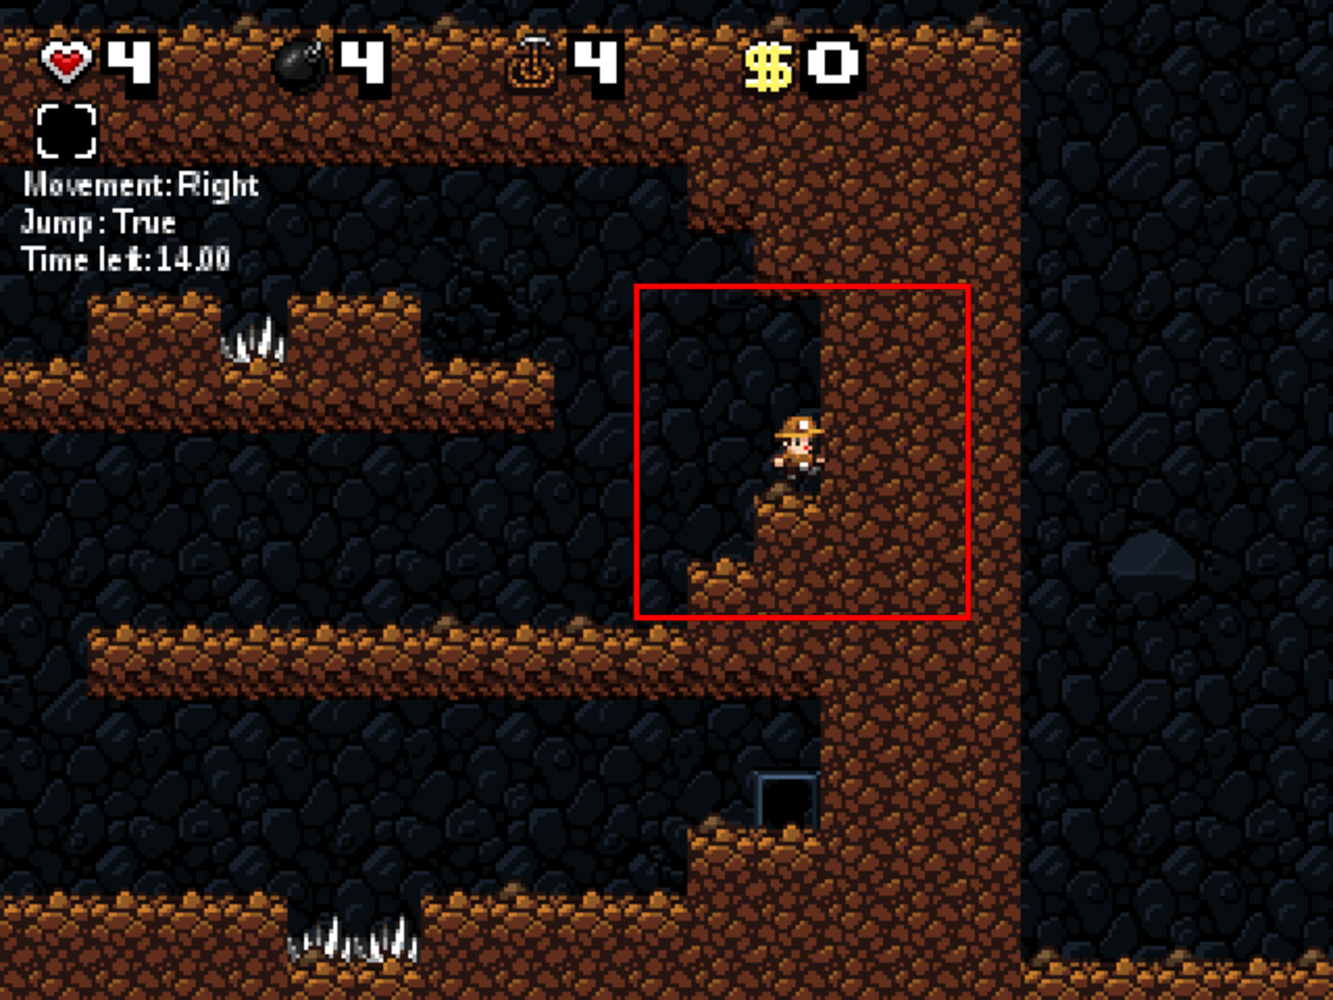
\includegraphics[width=.5\textwidth]{fig/experiment-medium-stuck.pdf}
\caption{Experimento mostrando o local onde o \textit{bot} fica parado ao
    executar no mapa médio com a média aritmética ponderada como função de
    aptidão.}
\label{fig:experiment-medium-stuck}
\end{figure}

Analisamos esse comportamento e percebemos que o \textit{bot} estava em um
local onde, naquele momento, ele considerava como \textit{ótimo}. Identificamos
isso pois nossa função de aptidão produz valores mais altos quanto maior for o
deslocamento horizontal e vertical do \textit{bot}. Dessa forma, caso ele fosse
para a esquerda, o valor de aptidão seria pior do que se ele ficasse parado
nesse local \textit{ótimo}. Um outro ponto importante é que é possível que as
mutações ou não estivessem ocorrendo ou não fossem suficientes para fazer com
que o \textit{bot} explorasse mais o mapa, de forma a fazer com que ele
entendesse que chegar na área inferior do mapa é mais vantajoso do que ficar
parado nesse local \textit{ótimo} por muitas gerações. O resultado dessa
execução pode ser visto na Figura \ref{fig:medium-wam-experiment}.

\begin{figure}[H]
\centering
	\begin{subfigure}[b]{0.4\textwidth}
        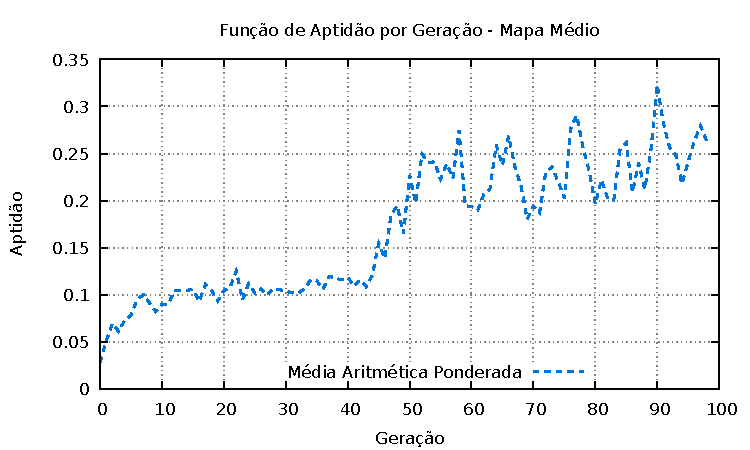
\includegraphics[width=\textwidth]{fig/medium-wam-fitness-experiment.pdf}
        \caption{Valor de aptidão em função do número de gerações para a média
        aritmética ponderada no mapa médio.}
	\end{subfigure}
	\begin{subfigure}[b]{0.4\textwidth}
        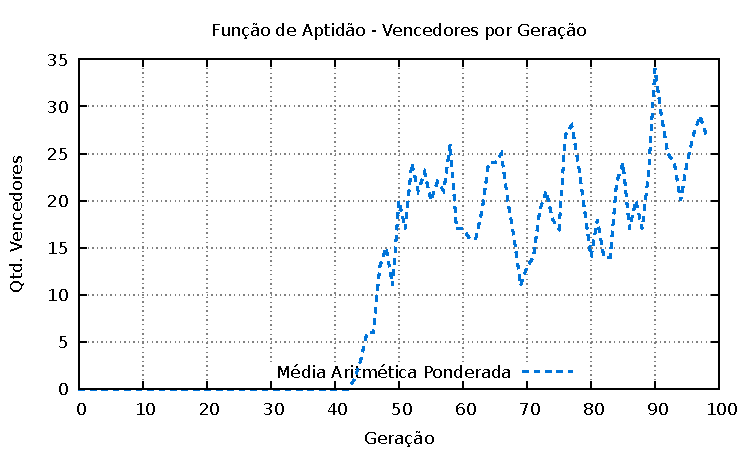
\includegraphics[width=\textwidth]{fig/medium-wam-winners-experiment.pdf}
        \caption{Número de organismos vencedores por geração para a média
        aritmética ponderada no mapa médio.}
	\end{subfigure}

    \caption{Resultado da execução do cenário médio com a média aritmética
    ponderada.}
	\label{fig:medium-wam-experiment}
\end{figure}

\todoin[caption={Citar capítulo de modelagem}] {
    Citar capítulo de modelagem.
}

Embora o \textit{bot} tenha vencido, ele demorou muito para isso -- após a
geração de número 40. Portanto, visando fazer com que ele aprendesse mais
rápido, adicionamos a entrada de \textit{obstáculo} na rede. O resultado dessa
modificação pode ser vista na Figura \ref{fig:medium-wam-obs-fitness-experiment}.

\begin{figure}[H]
\centering
	\begin{subfigure}[b]{0.4\textwidth}
        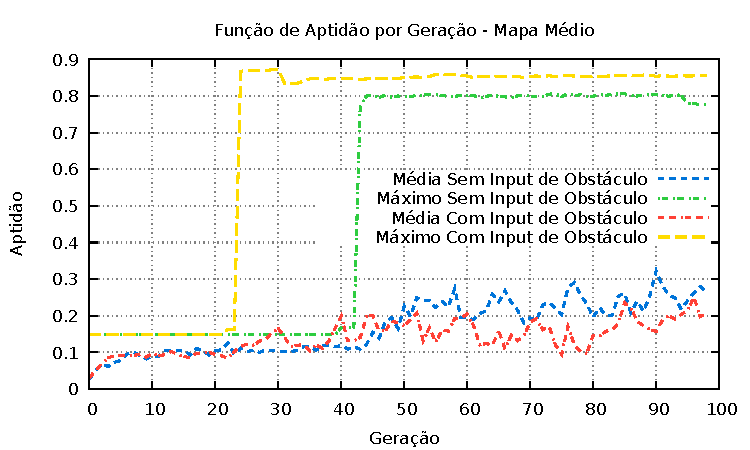
\includegraphics[width=\textwidth]{fig/medium-wam-obs-fitness-experiment.pdf}
        \caption{Valor de aptidão em função do número de gerações para a média
        aritmética ponderada, com o \textit{input} de obstáculo, no mapa
        médio.}
	\end{subfigure}
	\begin{subfigure}[b]{0.4\textwidth}
        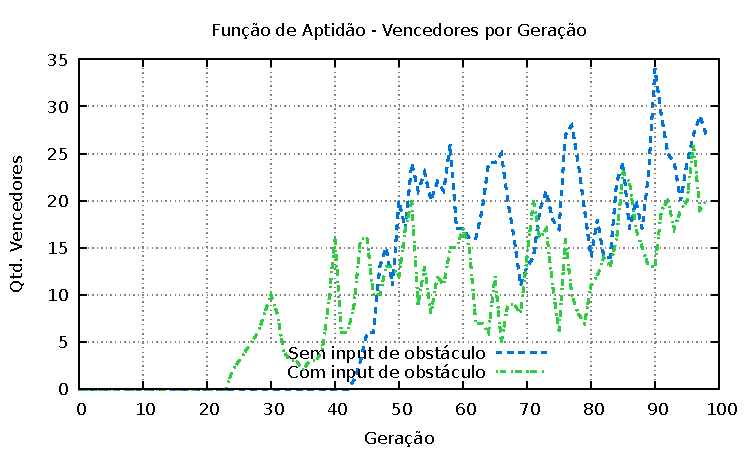
\includegraphics[width=\textwidth]{fig/medium-wam-obs-winners-experiment.pdf}
        \caption{Número de organismos vencedores por geração para a média
        aritmética ponderada, com o \textit{input} de obstáculo, no mapa
        médio.}
	\end{subfigure}

    \caption{Resultado da execução do cenário médio com a média aritmética
    ponderada.}
	\label{fig:medium-wam-obs-fitness-experiment}
\end{figure}

Concluímos então que a adição dessa nova entrada na rede melhorasse a execução
do \textit{bot}. Podemos ver isso pelo aumento no valor máximo da função nas
primeiras 30 gerações. Além disso, sem essa entrada, o bot levava em torno de
45 gerações para encontrar um organismo vencedor. Com ela, podemos ver que por
volta de 25 gerações já foi possível encontrar um organismo vencedor.

\subsection{\label{section:experiment-vision}Tamanho da Janela de Visão}

\todoin[caption={Janela de Visão: Aguardando Resultados}, color=red!80] {
    Aguardando resultados.
}

\subsection{Configurações de Mutação}

\todoin[caption={Configurações de Mutação: Aguardando Resultados},
color=red!80] {
    Aguardando resultados.
}

\subsection{Execução no Cenário \textit{extra 1}}

\todoin[caption={Cenários Extra 1: Aguardando Resultados}, color=red!80] {
    Aguardando resultados.
}

\begin{figure}[H]
\centering
	\begin{subfigure}[b]{0.4\textwidth}
        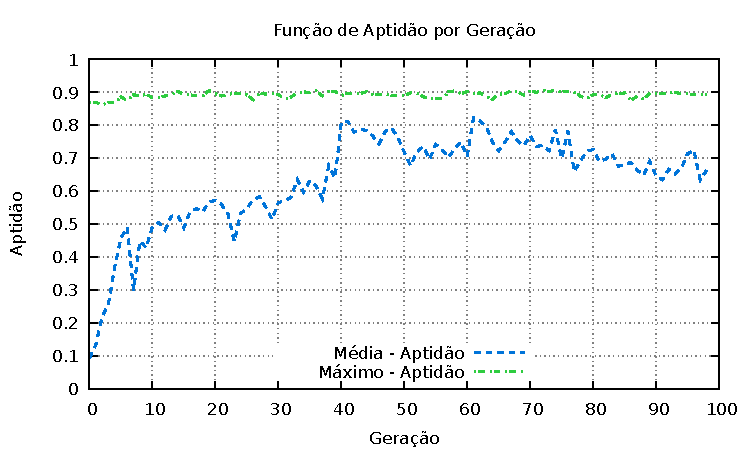
\includegraphics[width=\textwidth]{fig/extra1-fitness.pdf}
        \caption{Aptidão em função do número de gerações para o cenário
        \textit{extra 1}.}
	\end{subfigure}
	\begin{subfigure}[b]{0.4\textwidth}
        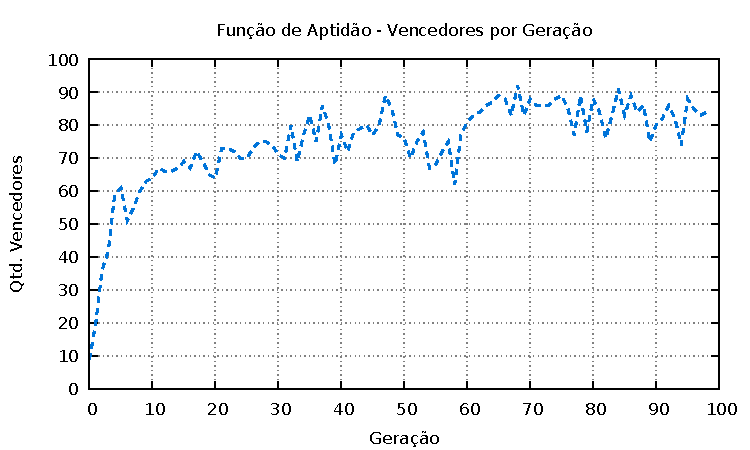
\includegraphics[width=\textwidth]{fig/extra1-winners.pdf}
        \caption{Número de organismos vencedores por geração para o cenário
        \textit{extra 1}.}
	\end{subfigure}

    \caption{Resultado da execução do cenário \textit{extra 1}.}
	\label{fig:extra1-results}
\end{figure}

\subsection{Execução no Cenário \textit{extra 2}}

\todoin[caption={Cenários Extra 2: Aguardando Resultados}, color=red!80] {
    Aguardando resultados.
}

\subsection{Execução no Cenário \textit{extra 3}}

\todoin[caption={Cenários Extra 3: Aguardando Resultados}, color=red!80] {
    Aguardando resultados.
}

\begin{figure}[H]
\centering
	\begin{subfigure}[b]{0.4\textwidth}
        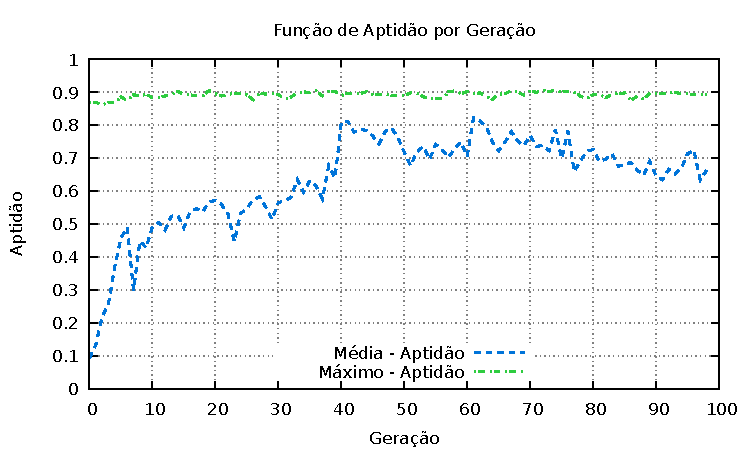
\includegraphics[width=\textwidth]{fig/extra1-fitness.pdf}
        \caption{Aptidão em função do número de gerações para o cenário
        \textit{extra 3}.}
	\end{subfigure}
	\begin{subfigure}[b]{0.4\textwidth}
        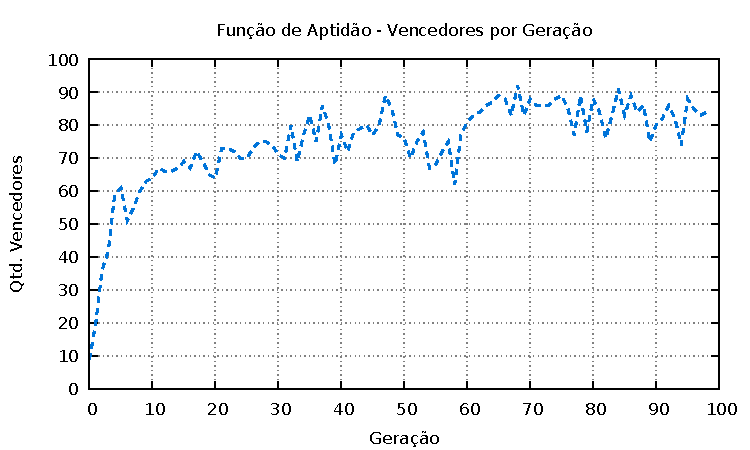
\includegraphics[width=\textwidth]{fig/extra1-winners.pdf}
        \caption{Número de organismos vencedores por geração para o cenário
        \textit{extra 3}.}
	\end{subfigure}

    \caption{Resultado da execução do cenário \textit{extra 3}.}
	\label{fig:extra3-results}
\end{figure}
